\documentclass[sigconf]{acmart}

\title{Infinite Jest: An Elegant Hairball}
\author{
  K. Hunter Wapman
  \and
  Brian Lubars
  \and
  Carl Mueller
}
\date{\today}

%\documentclass[12pt]{article}
%\usepackage[margin=1in]{geometry}
\usepackage{amsmath}
\usepackage{enumitem}
\usepackage{graphicx}
\usepackage{listings}
% \usepackage{physics}
% \usepackage{subfig}
\usepackage{hyperref}
\usepackage{graphicx} % for pdf, bitmapped graphics files
\usepackage{caption}
\usepackage{subcaption}
\usepackage{wrapfig}
\usepackage[font={small}]{caption}
\usepackage{csquotes}
\usepackage{placeins}
\usepackage{xspace}

%\renewcommand\thesubsection{\alph{subsection}}

\newcommand{\infinitejest}{{\em Infinite Jest}\xspace}

%remove stupid copyright info
\settopmatter{printacmref=false}
\setcopyright{none}
\makeatletter
\def\@copyrightspace{\relax}
\makeatother

\captionsetup[subfigure]{aboveskip=2pt,belowskip=-1pt}
\captionsetup[table]{aboveskip=2pt,belowskip=-1pt}
\captionsetup[figure]{aboveskip=4pt,belowskip=0pt}
\setlength{\dbltextfloatsep}{8pt}
\setlength{\dblfloatsep}{8pt}
\setlength{\floatsep}{6pt}
\setlength{\textfloatsep}{8pt}

\begin{document}
\maketitle

\section{Introduction}

Does a story mirror the world, or show a different one? How does a story's structure impact its narrative? We analyze David Foster Wallace's \infinitejest as a network in an attempt to answer variants of these two questions:

\begin{enumerate}
    \item Does the story's social network mirror the world or show a different one?
    \item Why did the author choose to structure the narrative out of chronological order?
\end{enumerate}

To do so, we extract a network of character interactions that grows as the book progresses and pursue analyses in two contexts:

\begin{enumerate}
    \item \textbf{Statically}: analyzing the state of the book's network at the time of its end. 
    \item \textbf{Dynamically}: analyzing the state of the book's network as it grows throughout the telling.
\end{enumerate}

\subsection{A mirror of the world?}

There is a complex social network of characters and their interactions in \infinitejest. We make qualitative comparisons of its network of characters and their interactions with those one could expect to find in real-world social networks and random graphs. 

We compare this narrative social network to properties exhibited by real-world networks, examining its degree distribution, inverse degree assortativity, and community structure.

We find that centrality measures -- degree centrality and betweenness specifically -- accurately identify important characters. 

We also explore gender bias in the network, an aspect of the book that has received significant criticism.

\subsection{How does structure impact narrative?}

In \infinitejest the world is revealed only in pieces and indirectly, and it is up to the reader to stitch those pieces together to create complete picture and to maintain a coherent view of the story as it progresses. 

It's a non-statement to say that a novel's structure impacts its narrative, but it is far from so easy to answer the question ``how?'' In an effort to answer this question quantitatively, we ask: ``does the decision to tell the story out of chronological order make it more or less comprehensible for the reader?'' and compare the dynamics produced by growing the network in the two orderings.

Our examination of the book's chronology leads us to a new understanding of the kinds of functions events in the book take on and encourages a distinction between events that expose the world (functioning as exposition), and those that drive the narrative forward.

\section{Background}

``Certain kind of parallel lines are supposed to start converging in such a way that an `end' can be projected by the reader somewhere beyond the right frame. If no such convergence or projection occured to you, then the book's failed for you.'' -- David Foster Wallace \cite{badger_internet_1996}

\subsection{The structure of \infinitejest}

\infinitejest's structure differs from that of a typical book in a number of ways.

\subsubsection{Chronology}

The story is made up of 192 sections which are ordered non-chronologically; as seen in figure~\ref{chronology_bars}, the first sections to occur in the book appear last chronologically.

\begin{figure}[ht]
    \centering
    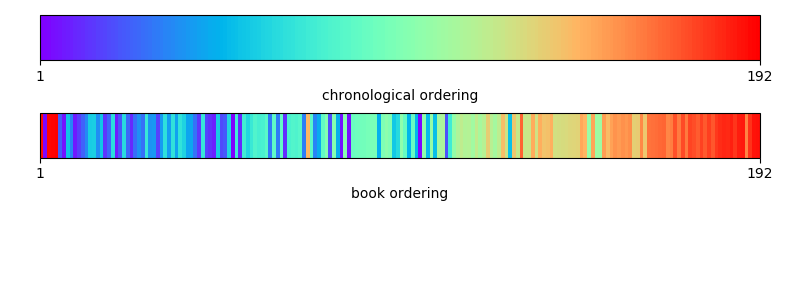
\includegraphics[width=.5\textwidth]{../data/plots/section_bars.png}
    \caption{Contrasting the ordering of events per the book with the chronology presented in \cite{carlisle_2007}}
    \label{chronology_bars}
\end{figure}

\subsubsection{Sierpinski Gasket}

The book's structure is ostensibly based on a Sierpinski Gasket, a triangular fractal.

\begin{figure}[ht]
    \centering
    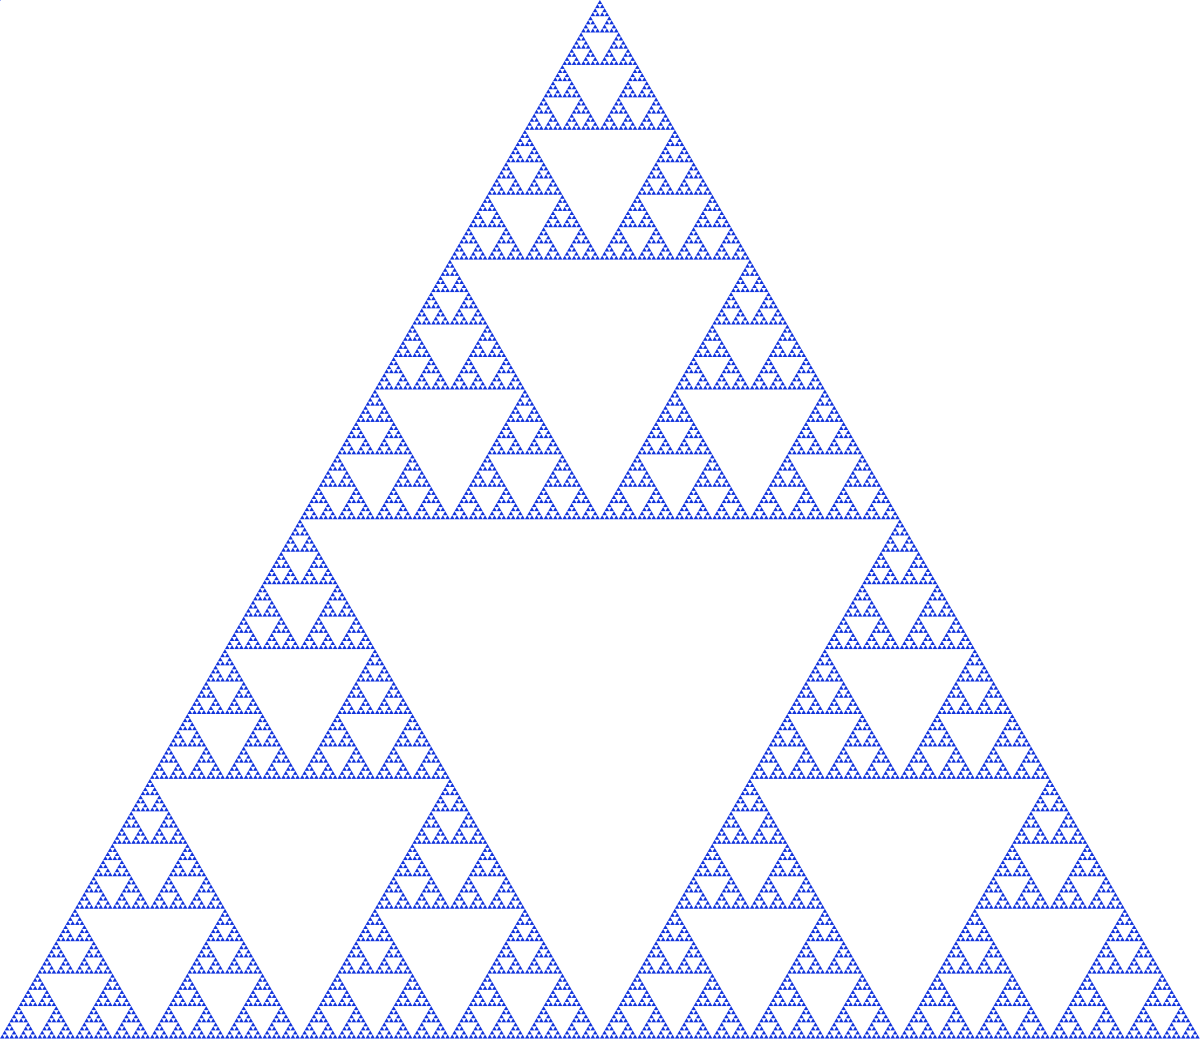
\includegraphics[width=.25\textwidth]{images/sierpinski.png}
    \caption{Sierpinski Gasket}
    \label{Sierpinski Gasket}
\end{figure}

\subsubsection{Endnotes}

The book uses endnotes extensively to convey additional information of varying degrees of relevance. The gamut of information can run from multi-page mini-stories containing important narrative information (\infinitejest, endnote 304) to ``No clue.'' (\infinitejest, endnote 216). Endnotes can reference other endnotes (\infinitejest, endnote 45), and can themselves have endnotes (\infinitejest, endnotes 388). These present a challenge both for the reader and for our approach to generating the network.

\section{\infinitejest as a Network}

Our network represents characters as nodes and character co-mentions as weighted edges. The more of often two characters are mentioned in proximity to each other, the greater the weight of the edge between them. Our approach gives an extremely broad view of a book as a network of character co-mentions.

Our choice of representing characters as nodes is fairly standard, but it worth noting that there are many possible definitions of an edge in a social network: character interaction, be it verbal (in dialogue) or physical, or sentiment. 

There are certainly drawbacks to our approach -- dynamics of power between characters are entirely omitted -- but we found it still allowed us to gain insight into narrative flow and characteristics of nodes.

\subsection{Network Design}

\subsubsection{Nodes}
Network nodes constitute characters identified in the set of found named entities. These were referenced against online resources to ensure proper coverage of the characters in the book.\cite{david_foster_wallace_wiki}

\subsubsection{Edges}
Edges in the book represent a co-mention between two entities in the text. We do not match across section breaks, and we directly interpolate endnotes into the sections in which they appear. We do not interpolate endnotes referenced in an endnote into that endnote.

A threshold number of tokens (words) under which the number of tokens between the mention of one entity and another determines if an edge with weight 1 is created. If the edge already exists, the weight is incremented by 1. The current entity $i$ is only matched with proceeding entities $j$ within this threshold.

The threshold number of tokens is determined by a heuristic measure of the effect of the threshold length on the average clustering coefficient and the giant component size (see Figure \ref{fig-threshold-size}). The intuition behind these metrics is to choose the minimum threshold required to produce a giant component and a clustering coefficient that captures the highly connected nature of characters in the novel. Our threshold is 50 tokens.

\begin{figure}[ht]
    \centering
    \begin{subfigure}{0.4\textwidth}
        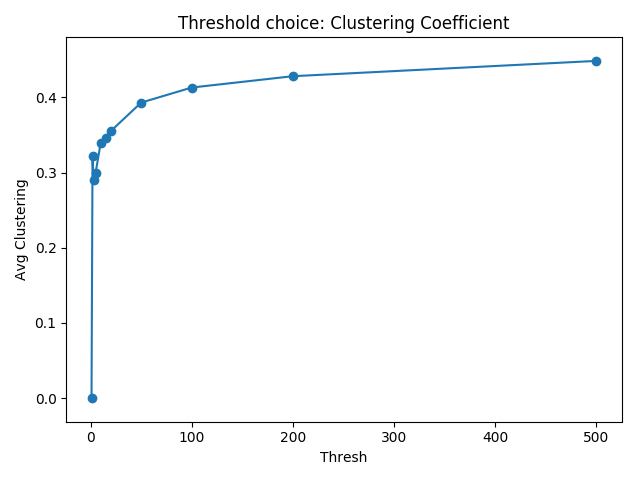
\includegraphics[width=1.\textwidth]{images/thresh_vs_avg_clustering.png}
        \caption{Edge Threshold's effect on Clustering Coefficient}
    \end{subfigure}
    \\
    \begin{subfigure}{0.4\textwidth}
        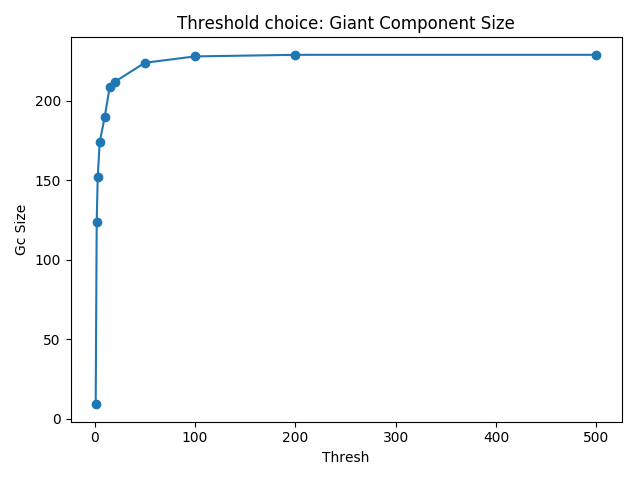
\includegraphics[width=1.\textwidth]{images/thresh_vs_gc_size.png}
        \caption{Edge Threshold's effect on the size of the Giant Component}
    \end{subfigure}
    \caption{Determining the Edge Threshold by its effect on clustering coefficient and the size of the Giant Component.}
    \label{fig-threshold-size}
\end{figure}

\subsubsection{Section as Snapshots and Modeling Recency}
In order to make comparisons between the book's ordering of events ('booktime') and the chronological ordering, we constructed a timelapse of graph snapshots that represents the aggregate graph structure up to the current section in the given ordering. Regardless of the ordering, the graph at the end of each sequence is identical. To model the differences in exposure to narratives and characters between the two orderings, we add a mechanism to decay the weights of the graph. Whenever a section is applied to the cumulative network, that section's weights are passed through a decay function orginially developed by psychologist Hermann Ebinghaus dubbed a `forgetting curve'. This curve is as follows:

\begin{equation}
    R = e^{\frac{-t}{(10000*s)}}
\end{equation}

Here $R$ represents the memory retention. $t$ represents the time (the number of tokens in the section). $s$ represents memory stability. The exponent is scaled by $\frac{1}{10000}$ to ensure reasonable memory retention values between $0$ and $1$. This approach enables us build a rough model the decaying memory of a reader to the narrative and character exposure differences between `chronological' and `booktime' section orderings.

\subsection{Network Design}

\begin{figure*}[t]
    \centering
    \begin{subfigure}{0.4\textwidth}
        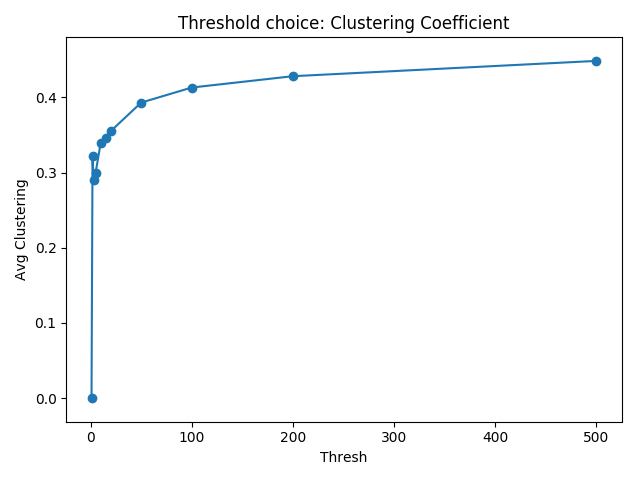
\includegraphics[width=1.\textwidth]{images/thresh_vs_avg_clustering.png}
        \caption{Clustering Coefficient vs. Threshold Size}
    \end{subfigure}
    ~
    \begin{subfigure}{0.4\textwidth}
        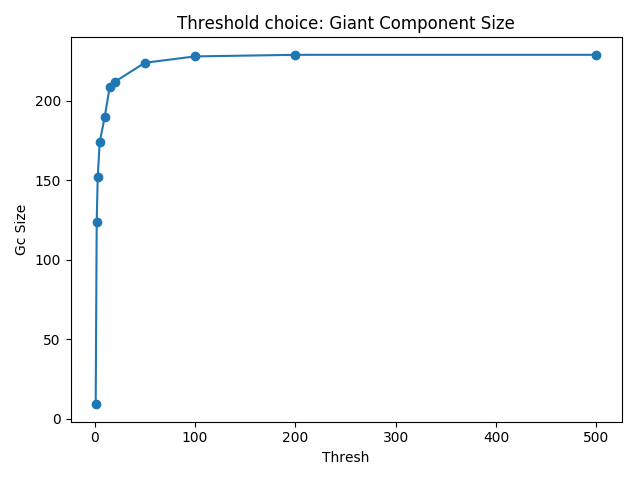
\includegraphics[width=1.\textwidth]{images/thresh_vs_gc_size.png}
        \caption{Giant Component Size vs. Threshold Size}
    \end{subfigure}
    \caption{Comparing threshold size effect on clustering coefficient and giant component size in order to determine the ideal threshold size.}
    \label{fig-threshold-size}
\end{figure*}

\subsubsection{Nodes and Edges}
Network nodes constitute each character identified in the set of found named entities. These were referenced against online resources to ensure proper coverage of the characters in the book. Edges in the book represent a co-mention between two entities in the text. A threshold number of tokens (words) under which the number of tokens between the mention of one entity and another determines if an edge is established. If the edge already exists, the weight is updated by adding `1' to the current weight value. The current entity $i$ is only matched with proceeding entities $j$ within this threshold. Once no match is found, the next available entity is checked for proceeding matches.

The threshold number of tokens is determined by a semi-objective measure of the effect of the threshold length on the average clustering coefficient and the giant component size (see Figure \ref{fig-threshold-size}). The intuition behind the use of these metrics is that we choose the minimum threhold length required to produce a large giant component and ample enough clustering best capturing the highly connected nature of characters in the novel. Our chosen threshold is 50 tokens.

\subsubsection{Section Snapshots and Modeling Recency}
One of the major considerations of our analyses concerns the ordering of sections. The book does not follow a chornological ordering with contiguous secitons potentially taking place anywhere within the time range of the book. However, the book Elegant Complexity \cite{carlisle_2007} provides a chronological ordering of sections. To perform a comparison of these two orders (`chronological' and `'booktime'), we constructed a timelapse of graph snapshots that represents the aggregate graph structure up to the current section in the given ordering. 

Regardless of the ordering, the graph at the end of each sequence will be identical. To model the differences in exposure to narratives and characters between the two orderings, we perform a decay mechanism of the weights of the graph. At each section, the corresponding graph snapshot's weights are mapped through a decay function developed orginially by psychologist Hermann Ebinghaus dubbed a `forgetting curve' \cite{murre2015replication}. This curve is as follows:


\begin{equation}
    R = e^{\frac{-t}{(10000*s)}}
\end{equation}


Here $R$ represents the memory retention. $t$ represents the time, which we measure using the number of tokens per section. $s$ represents memory stability. The exponent is scaled by $\frac{1}{10000}$ to ensure reasonable memory retention values between $0$ and $1$. This approach enables us build a rough model the decaying memory of a reader to the narrative and character exposure differences between `chronological' and `booktime' section orderings.

\section{Static-Network Analysis}

\subsection{Statistics}

\subsection{Small World}
At the book's end, the largest component has 224 nodes and the diameter is 5.
Since $ln(224) = 5.41$, we see that this network does indeed display the small world property, similar to real-world social networks.

\subsection{Degree Distribution}

\begin{figure}[ht]
    \centering
    \begin{subfigure}{0.4\textwidth}
        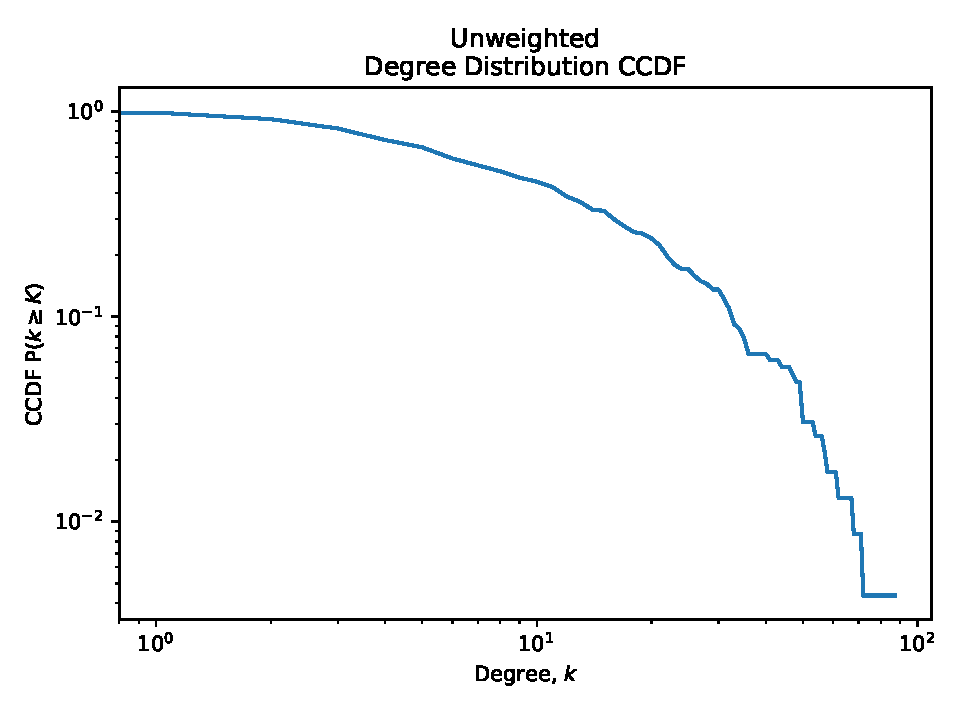
\includegraphics[width=1.\textwidth]{images/unweighted_degree_distr_ccdf.pdf}
        \caption{Unweighted degree distribution.}
    \end{subfigure}
    \begin{subfigure}{0.4\textwidth}
        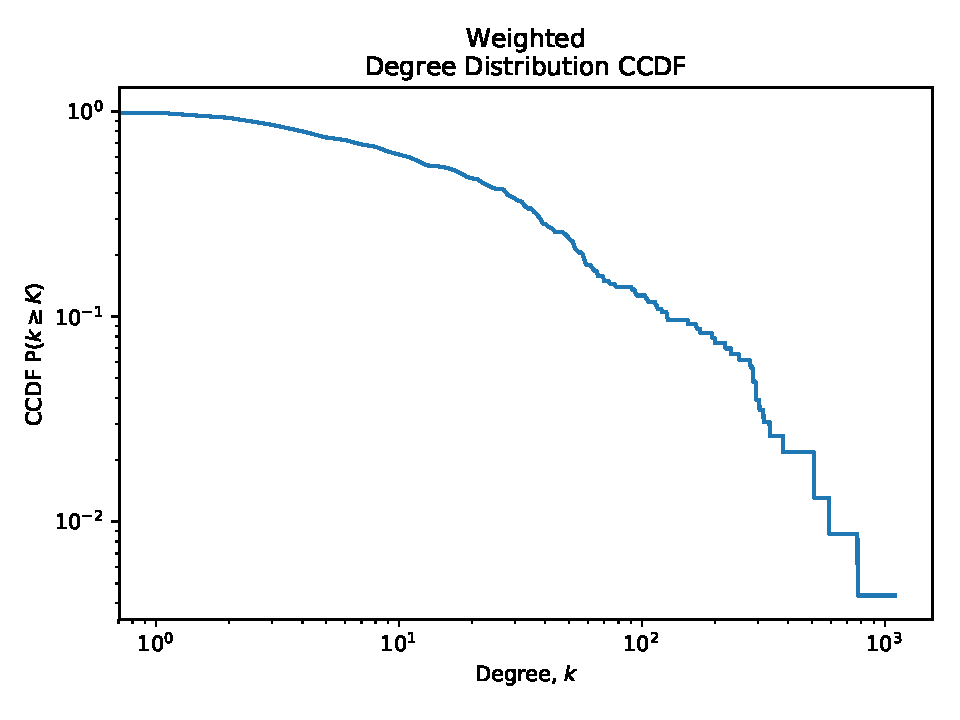
\includegraphics[width=1.\textwidth]{images/weighted_degree_distr_ccdf.pdf}
        \caption{Weighted degree distribution.}
    \end{subfigure}
    \caption{Degree distributions on a log-log scale. Though we do observe a heavy tail, we do not see a power law.}
    \label{fig:degree_distr}
\end{figure}

The degree distributions for the weighted and unweighted networks are shown as a CCDF in Figure \ref{fig:degree_distr}. We see a heavy tail like we might expect from many real-world networks, but neither appear to show a power law in the tail. 

In the unweighted network in particular we see a distribution that clearly has more high-degree nodes than expected under a Poisson random graph, yet the tail drops of much faster than expected in a scale-free network.
The weighted degree distribution shows a heavier tail than the unweighted one, suggesting the distribution of character mentions within the book is much more uneven than the unweighted graph of character interactions. The weighted network is closer to a power law, though we still hesitate to call it scale-free.

%$P(k) \sim k^{-\tau}$, or power law with a cutoff, $P(k) \sim k^{-\tau}10^{-k/c}$

We can only speculate on the attachment mechanism behind the degree distribution, leaving testing such hypothesis to future work. Since the degree distribution does not follow a power law, vertex copying and preferential attachment do not make sense. 
Perhaps main characters are introduced in the beginning, and the book does not contain many minor throw-away characters.

The average degree is 13.31 and the average weighted degree is 55.95

\subsection{Assortativity}
We see an unweighted degree assortative mixing coefficient of -0.0945.
Degree assortative networks typically reflect core-periphery structures, where a dense core of highly-connected nodes is surrounded by successively less-dense periphery nodes. Degree disassortative networks, on the other hand, are more stars with high-degree nodes connected to low-degree. 
According to Newman in {\em Networks}, social networks are unusual in that they typically have a positive degree assortativity \cite{NewmanBook}. 
Therefore it is strange for us to see disassortative mixing by degree in \infinitejest, possibly indicating more of a star-like structure or fewer community structures than real-world social networks.

\subsection{Modularity}

- talk about NMI
- talk about modularity

\subsection{Clustering}
Using the transitivity definition of clustering coefficient, we can examine the fraction of closed triads.
$$ C = \frac{\text{(number of triangles)} \cdot 3}{\text{number of connected triples}} $$

This metric disregards the edge weights, looking only at connections between characters. We find $C = 0.3930$, reflecting the relatively dense connections -- perhaps within communities such as the Tennis Academy or Halfway House -- as opposed to a tree-like structure rooted at the highest-degree (main) characters.

We can compare the clustering coefficient against the configuration model to determine if this effect is due to the degree sequence alone or perhaps reflects a conscious author choice. We find configuration model we get an average local clustering coefficient of 0$.1728$, vs $0.3930$ in the book. 

TODO: how does this compare to real social networks?

\subsection{Gender}


\section{Dynamic Analysis}

\subsection{Narrative}

We hypothesized that the book would be easier to understand when structured chronologically, but our analysis does not bear this out. As shown by figure~\ref{component-sizes}-A, while there are at most $12$ disconnected plot-lines in the original book order, there are as many as 19 disconnected plot-lines in the first quarter of the chronologically ordered book. It is quite a challenge to keep track of $12$ unrelated plot lines; the idea of keeping track of $19$ in Wallace's convoluted text is boggling. This makes it clear that the events in the book that occur out of chronological order provide context, and function as expositions that stitch together disparate components of the character network. On the other hand, those sections that appear chronologically provide \infinitejest's narrative structure and move the novel's plot forward.

Figure~\ref{component-sizes}-B shows that in both the booktime and the chronological orderings, the growth of the size of the largest component slows around section 75, mirroring the point in figure~\ref{component-sizes}-A where the number of components takes a steep decline, indicating that at this point in the novel, most of the important characters have been introduced, and most of the plot lines have entered the story proper.

\begin{figure}[ht!]
    \centering
    \begin{subfigure}{0.4\textwidth}
        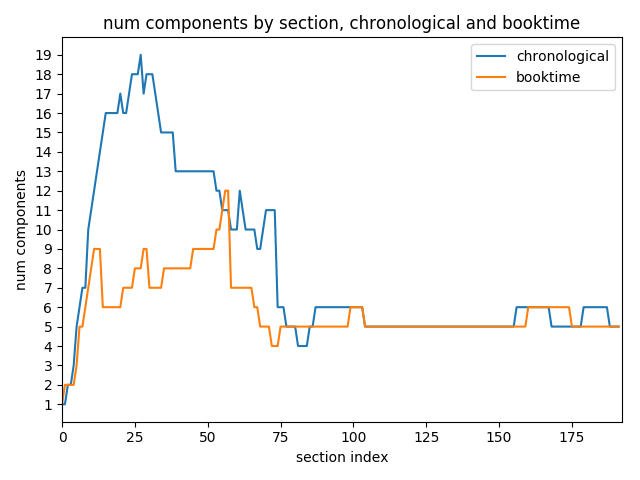
\includegraphics[width=1.\textwidth]{images/dynamics-num-components.png}
        \caption{Number of components as a function of section}
    \end{subfigure}
    \begin{subfigure}{0.4\textwidth}
        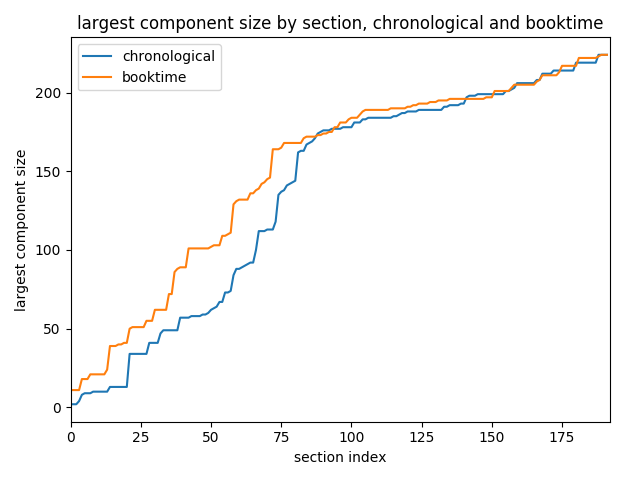
\includegraphics[width=1.\textwidth]{images/dynamics-largest-components.png}
        \caption{Largest component size as a function of section}
    \end{subfigure}
    \caption{Number of components and largest component size as a function of section}
    \label{component-sizes}
\end{figure}

\subsection{Sparsification vs Densification}

Does the growth of the story's display tendencies of sparsification (like an Erdos-Reyni random network, where relatively few edges are added for each new node) or of densification (where new nodes tend to add edges that complete triads)?

Figure \ref{sparsification-densification}-A shows that in both the chronological and booktime orderings, the mean geodesic path length increases until around $\frac{2}{3}$'s of all nodes have been added, at which point the mean geodesics path lengths decrease. In other words, both orderings generate a network that first sparsifies and later densifies. It is worth noting that the mean geodesic path length in the chronological ordering both grows more quickly and achieves a higher maximum value than the booktime ordering, displaying behavior more similar to a random network than the booktime ordering. This supports the idea that the chronological ordering creates more narrative fragmentation than the booktime ordering.

Figure~\ref{sparsification-densification}-B supports the idea of sparsification followed by densification. The average unweighted degree in the largest component following the same timeline as figure~\ref{sparsification-densification}-A -- where new nodes tend not to increase the mean degree (displaying sparsification) until around $\frac{2}{3}$'s of all nodes have been added, at which point new nodes tend to increase the mean degree (displaying densification).

\begin{figure}[ht]
    \centering
    \begin{subfigure}{0.4\textwidth}
        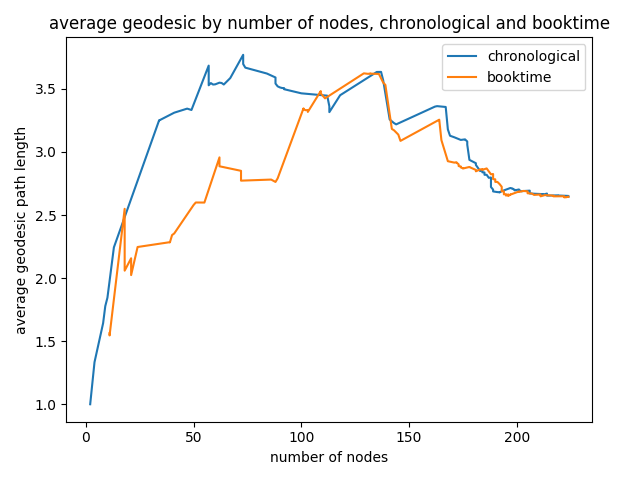
\includegraphics[width=1.\textwidth]{images/n_vs_geodesic-weighted_False.png}
        \caption{Mean geodesic path length in the largest component as a function of nodes}
    \end{subfigure}
    \begin{subfigure}{0.4\textwidth}
        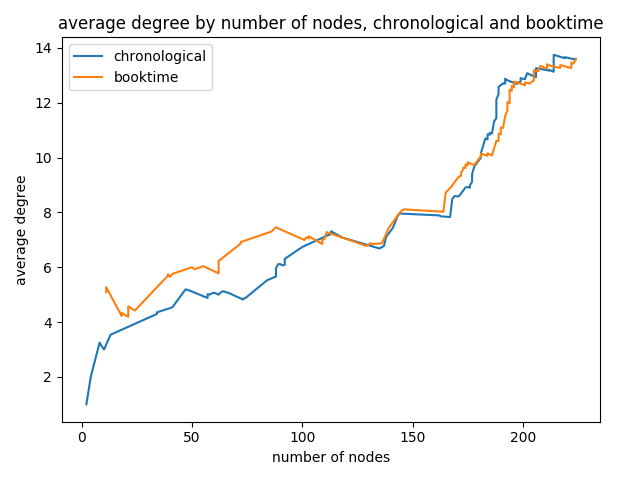
\includegraphics[width=1.\textwidth]{images/n_vs_avg_degree-weighted_False.png}
        \caption{Average unweighted degree in the largest component as a function of nodes}
    \end{subfigure}
    \caption{Node number's effect on average unweighted degree and mean geodesic path length in the largest component}
    \label{sparsification-densification}
\end{figure}



\section{Conclusion}

\bibliographystyle{ACM-Reference-Format}
\bibliography{references.bib}


\end{document}
